\chapter{Functional safety in embedded systems}
\label{functional_safety}

\section{Related standards}

A variety of standards exist for specific or general markets, to facilitate the compliance of systems to the functional safety principles. The standard IEC 61508 gives methods on how to apply, design, deploy and maintain automatic protection systems called safety-related systems.
Along with the more general standard, industry-specific standards exist:
\begin{itemize}

    \item ISO 26262 for automotive passenger vehicles,
    \item IEC 61511 for the process industry and associated instrumentation,
    \item EN 50128 for software development of railway applications,
    \item IEC 61513 for nuclear power plants,
    \item IEC 62061 and ISO 13849 for machinery electrical control systems,
    \item IEC 62304 for medical systems and
    \item IEC 60730 for white goods.

\end{itemize}

The mentioned standards provide guidelines to assess risk and assign safety goals for safety-related systems of various industries. They provide frameworks for quantitative analysis of random failure rates and the effectiveness of diagnostics to detect them. They also provide guidelines for maintenance of the safety-related systems after the deployment.

IEC 61508 is an umbrella functional safety standard applicable to all industries. It defines functional safety as: “Part of the overall safety relating to the EUC (Equipment Under Control) and the EUC control system which depends on the correct functioning of the Electrical/Electronic/Programmable Electronic Safety-related Systems (E/E/PE) safety-related systems, other technology safety-related systems and external risk reduction facilities.” The fundamental concept is that any safety-related system must work correctly or fail in a predictable (safe) way. Functional safety relies on active systems, and safety measures that rely on passive systems are not functional safety \citep{func_safety_explained}. 

\section{Terminology}

IEC 61508 standard introduces a lot of three-letter acronyms. This section covers the most common ones.

\subsection{SIL}

SIL or safety integrity level is a discrete level (one out of four) for specifying the safety integrity retirements of the safety instrumented functions (SIF) to be allocated to the safety instrumented system (SIS) i.e. SIL says how well the safety integrity function does its job. SIF and SIS are explained in \autoref{sec:sif}  and \autoref{sec:sis} respectfully. SIL of 1 marks the lowest safety integrity level and level 4 denotes the highest.  \autoref{fig:sil_level_chart} demonstrates that SIL is a function of the frequency of a hazard and the severity of the consequence. 


\begin{figure}[H]

      \centering
      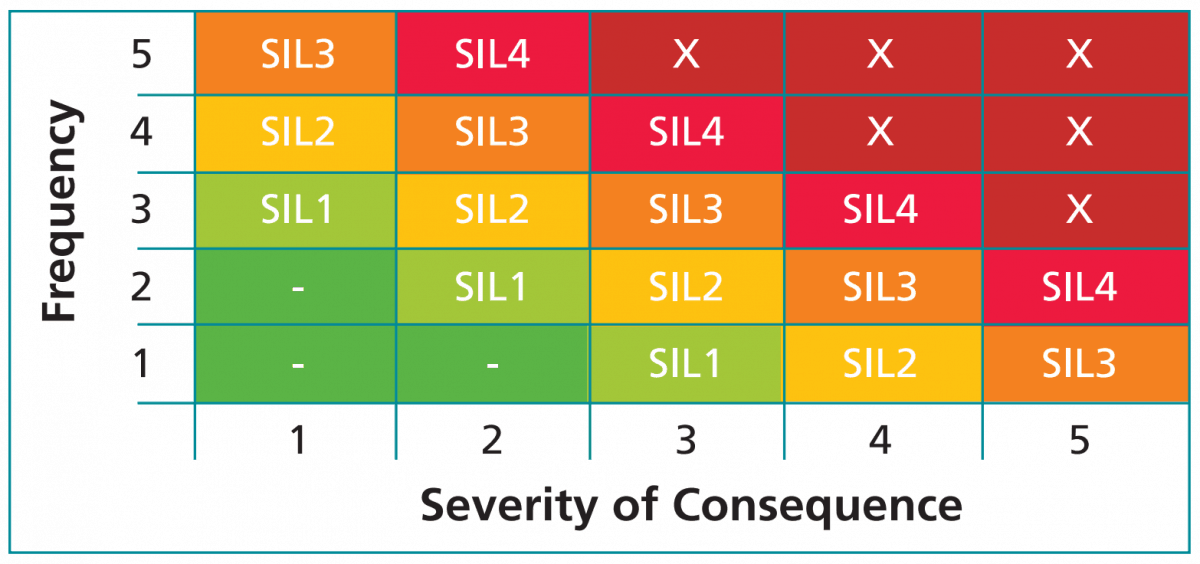
\includegraphics[width=0.7\linewidth]{images/sil_level_chart.png}
      \caption{Generic SIL chart as a function of severity and frequency}
      \label{fig:sil_level_chart}
    
\end{figure}

\subsection{SIF}
\label{sec:sif}

Safety instrumented function (SIF) is a set of equipment used to implement an automatic protection function. Safety function shall have a specified SIL to achieve functional safety. 
An example of SIF is a number of sensors looking for the one \textbf{single} hazard scenario. Those sensors need to bring the system to a safe state if the hazard occurs. SIF is usually measured in how much risk can be removed. It is usually expressed in either in PFDaverage or in SIL. 

\subsection{SIS}
\label{sec:sis}

SIS or safety instrumented system is one or more safety functions put together to do the whole job. SIS can encompass multiple different functions and act in multiple different ways to overcome a number of hazard scenarios, as opposed to SIF that can only perform one action to overcome one hazard scenario.

\section{Certification}


For the certification, the system integrity level is determined. SIL of a product is determined by three things \citep{func_safety_fundamentals}:
\begin{itemize}

    \item the systematic capability rating,
    \item the architectural constrains for the element and
    \item the PFDaverage calculation.
    
\end{itemize}

\begin{figure}[H]

      \centering
      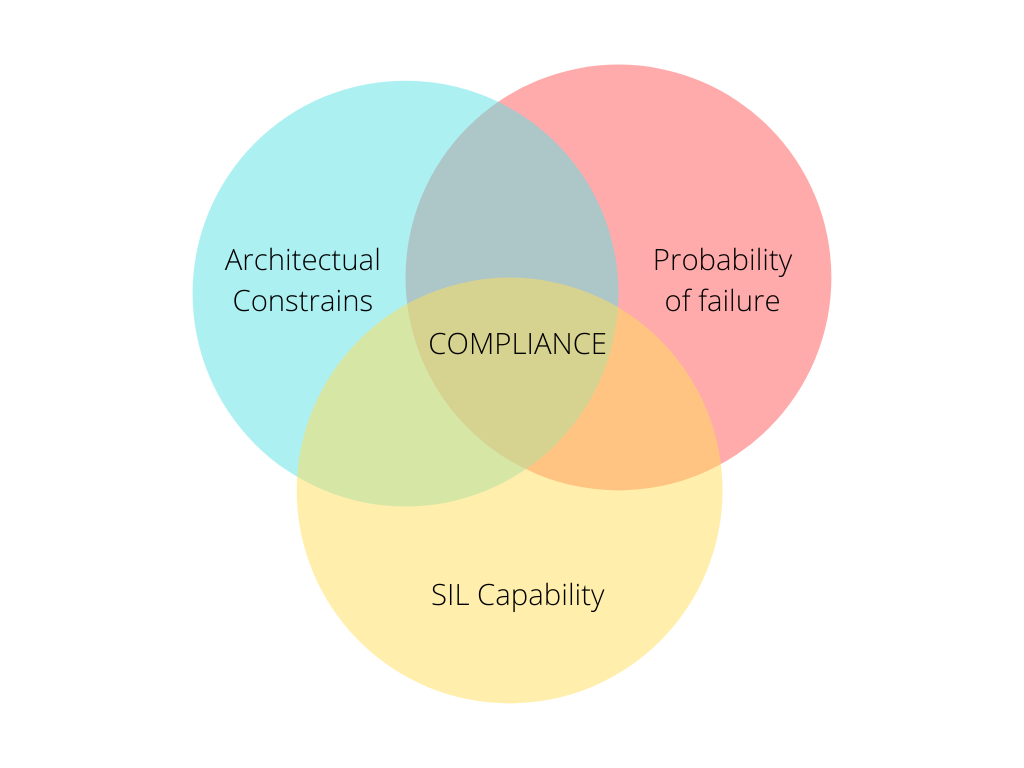
\includegraphics[width=0.7\linewidth]{images/sil_requirements.png}
      \caption{SIL requirements}
      \label{fig:sil_requirements}
    
\end{figure}

Systematic Capability is achieved when the equipment used to implement any safety function is designed using procedures intended to prevent systematic design errors.  The rigor of the required procedure is a function of a Safety Integrity Level (SIL). This is evaluated through an assessment of the quality management system for suppliers of process control and instrumentation for safety against the requirements in IEC 61508.  If the QMS meets the requirements of 61508 a SIL Capability rating is issued. 

Architectural constraints are estimated by the route 1H or route 2H as mentioned in IEC 61508. Route 1H is estimated by safe failure fraction(SFF). SFF is a percentage of safe failures in all failures. Route 2H is an assessment of the reliability data for the entire element according to IEC 61508. It is mostly based around the historical data of a device and is based on a method that demands 90 percent confidence in the data.  Instead of the SFF calculation, the Minimum Hardware Fault Tolerance is determined by a set of rules from IEC 61508.

Probability of Failure on Demand average (PFDaverage) is the probability that a system will fail dangerously, and not be able to perform its safety function when required. PFD can be determined as an average probability or maximum probability over a time period.

As mentioned before, a safety instrumented function needs to take the risk out of the system. If there is no requirement to reduce risk than a function doesn't need a SIL rating or, for that matter, functional safety. When a function still needs to reduce risk after the process hazard assessment (PHA), SIL needs to be incorporated. The tables below give a link between SIL and expected safety.

PFD (probability of dangerous failure) and RRF (risk reduction factor) of low demand operation for different SILs as defined in IEC 61508 are shown in \autoref{tab:func_safety_table_low_demand}.

\begin{table}[H]
\centering
\resizebox{0.7\textwidth}{!}{%
\begin{tabular}{
>{\columncolor[HTML]{FFFFFF}}l 
>{\columncolor[HTML]{FFFFFF}}l 
>{\columncolor[HTML]{FFFFFF}}l 
>{\columncolor[HTML]{FFFFFF}}l }
\hline
\multicolumn{1}{c}{\cellcolor[HTML]{FFFFFF}{\color[HTML]{202122} \textbf{SIL}}} &
  \multicolumn{1}{c}{\cellcolor[HTML]{FFFFFF}{\color[HTML]{202122} \textbf{PFD}}} &
  \multicolumn{1}{c}{\cellcolor[HTML]{FFFFFF}{\color[HTML]{202122} \textbf{PFD (power)}}} &
  \multicolumn{1}{c}{\cellcolor[HTML]{FFFFFF}{\color[HTML]{202122} \textbf{RRF}}} \\ \hline
{\color[HTML]{202122} 1} & {\color[HTML]{202122} 0.1-0.01}       & {\color[HTML]{202122} $10^{-1} - 10^{-2}$} & {\color[HTML]{202122} 10-100}         \\
{\color[HTML]{202122} 2} & {\color[HTML]{202122} 0.01-0.001}     & {\color[HTML]{202122} $10^{-2} - 10^{-3}$} & {\color[HTML]{202122} 100-1000}       \\
{\color[HTML]{202122} 3} & {\color[HTML]{202122} 0.001-0.0001}   & {\color[HTML]{202122} $10^{-3} - 10^{-4}$} & {\color[HTML]{202122} 1000-10,000}    \\
{\color[HTML]{202122} 4} & {\color[HTML]{202122} 0.0001-0.00001} & {\color[HTML]{202122} $10^{-4} - 10^{-5}$} & {\color[HTML]{202122} 10,000-100,000} \\ \hline
\end{tabular}%
}
\caption{Link between SIL, PFH and RRF for low demand operation}
\label{tab:func_safety_table_low_demand}
\end{table}

For continuous operation, \autoref{tab:func_safety_table_continuous} is provided (PFH - Probability of dangerous failure per hour).

\begin{table}[H]
\centering
\resizebox{0.9\textwidth}{!}{%
\begin{tabular}{
>{\columncolor[HTML]{FFFFFF}}l 
>{\columncolor[HTML]{FFFFFF}}l 
>{\columncolor[HTML]{FFFFFF}}l 
>{\columncolor[HTML]{FFFFFF}}l }
\hline
\multicolumn{1}{c}{\cellcolor[HTML]{FFFFFF}{\color[HTML]{202122} \textbf{SIL}}} &
  \multicolumn{1}{c}{\cellcolor[HTML]{FFFFFF}{\color[HTML]{202122} \textbf{PFH}}} &
  \multicolumn{1}{c}{\cellcolor[HTML]{FFFFFF}{\color[HTML]{202122} \textbf{PFH (power)}}} &
  \multicolumn{1}{c}{\cellcolor[HTML]{FFFFFF}{\color[HTML]{202122} \textbf{RRF}}} \\ \hline
{\color[HTML]{202122} 1} & {\color[HTML]{202122} 0.00001-0.000001}       & {\color[HTML]{202122} $10^{-5} - 10^{-6}$} & {\color[HTML]{202122} 100,000-1,000,000}         \\
{\color[HTML]{202122} 2} & {\color[HTML]{202122} 0.000001-0.0000001}     & {\color[HTML]{202122} $10^{-6} - 10^{-7}$} & {\color[HTML]{202122} 1,000,000-10,000,000}      \\
{\color[HTML]{202122} 3} & {\color[HTML]{202122} 0.0000001-0.00000001}   & {\color[HTML]{202122} $10^{-7} - 10^{-8}$} & {\color[HTML]{202122} 10,000,000-100,000,000}    \\
{\color[HTML]{202122} 4} & {\color[HTML]{202122} 0.00000001-0.000000001} & {\color[HTML]{202122} $10^{-8} - 10^{-9}$} & {\color[HTML]{202122} 100,000,000-1,000,000,000} \\ \hline
\end{tabular}%
}
\caption{Link between SIL, PFH and RRF for continuous operation}
\label{tab:func_safety_table_continuous}
\end{table}

When a safety instrumented function fulfills the aforementioned SIL requirements a certified can be assigned for the SIL. Example of a certificate is given in \autoref{fig:func_safety_certificate}.

\begin{figure}[H]

      \centering
      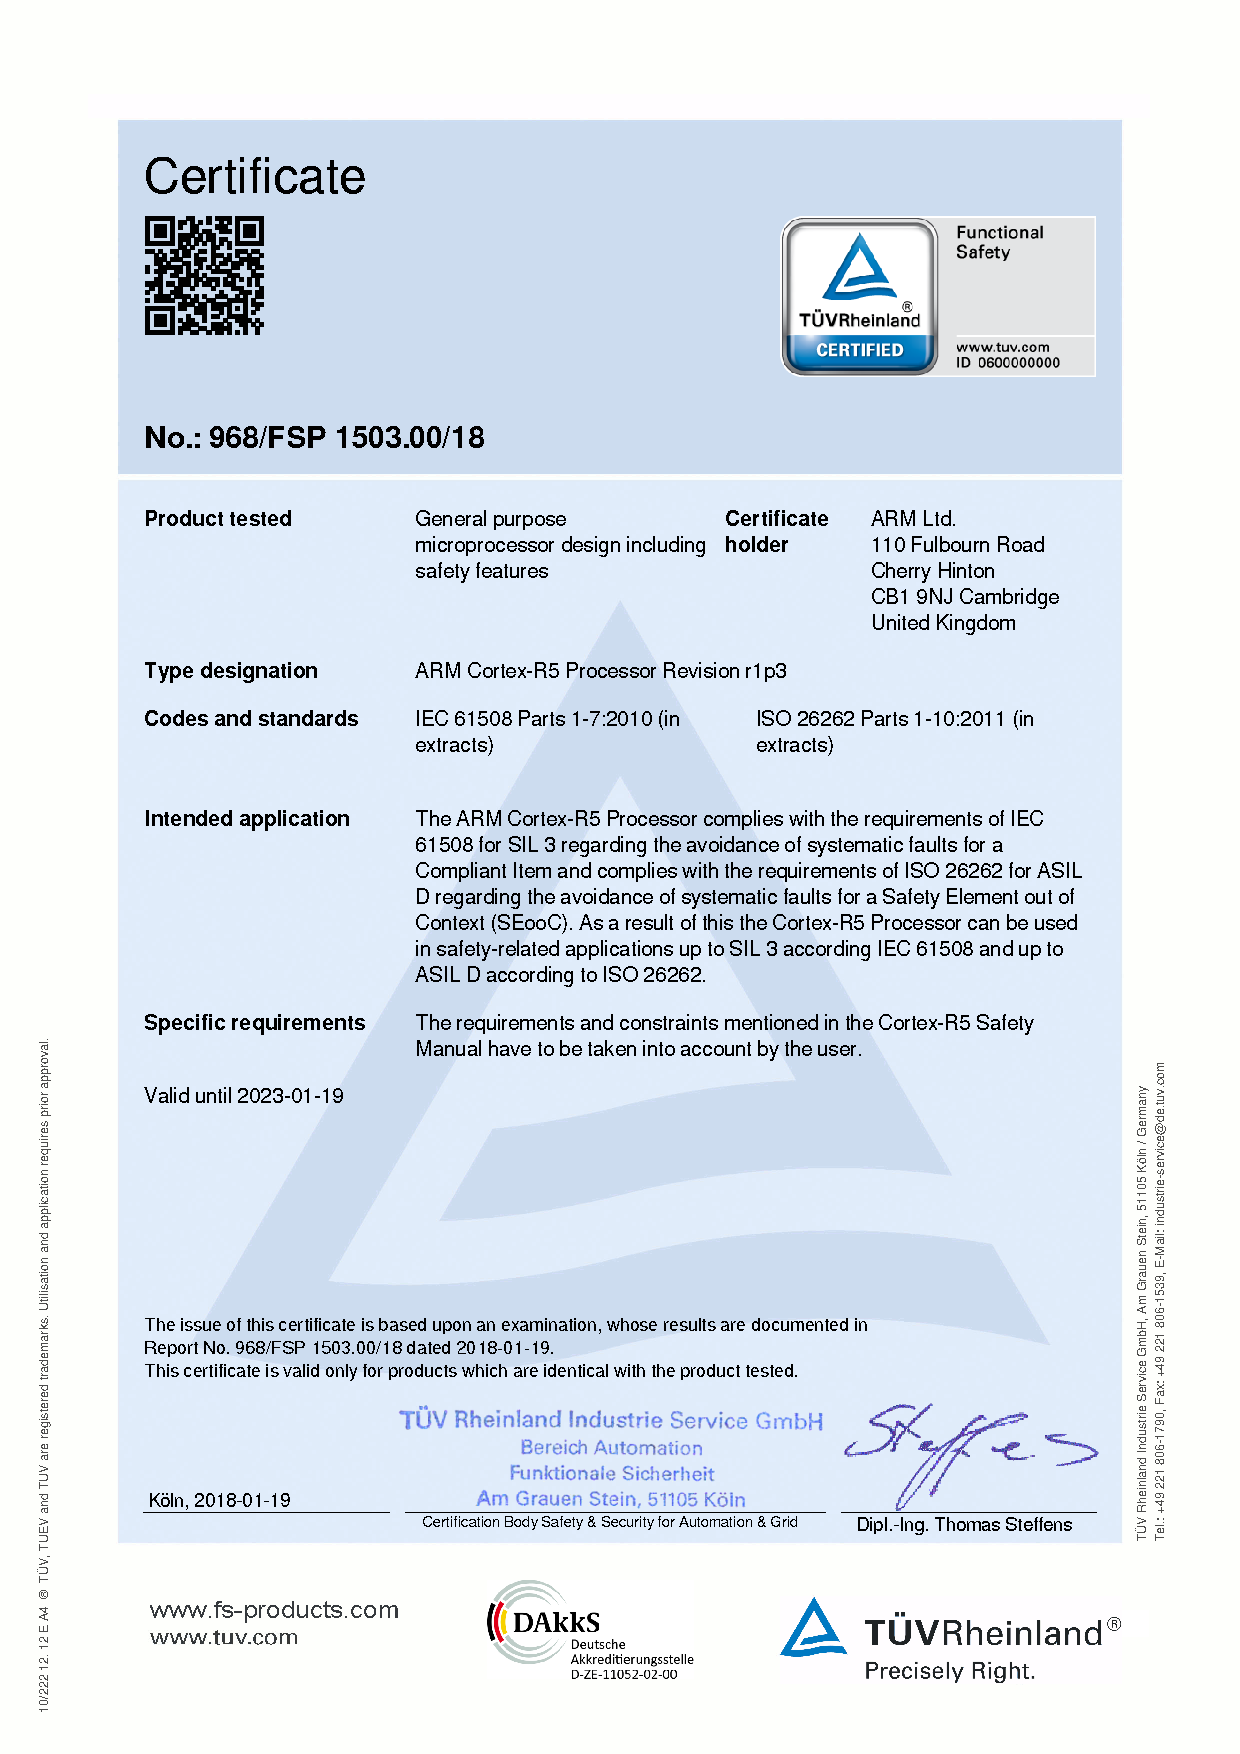
\includegraphics[width=0.9\linewidth]{images/cortex_r_certificate.pdf}
      \caption{ARM Cortex-R5 Processor  SIL 3 certificate}
      \label{fig:func_safety_certificate}
    
\end{figure}

\section{Embedded processors redundancy - lockstep}

\subsection{Introduction}

Consider a system with one processing unit. Such a system is obviously non-redundant from the
aspect of instruction execution. Lockstep is a redundancy mechanism for increasing the system reliability
by introducing at least one redundant processing unit. The redundant processing unit replicates the behavior of
the original processing unit. Depending on the number of processing units lockstep can provide fault-detection, if there are less than three processing units in a system, or both fault-detection and
fault-tolerance with more than two processing units in a system \citep{ipavic_lockstep}. \autoref{fig:patent_not_delayed} shows CPU1 and CPU2 in lockstep. CCU or CPU compare unit compares the outputs from the CPUs and throws an error if there is a mismatch.

\begin{figure}[H]

      \centering
      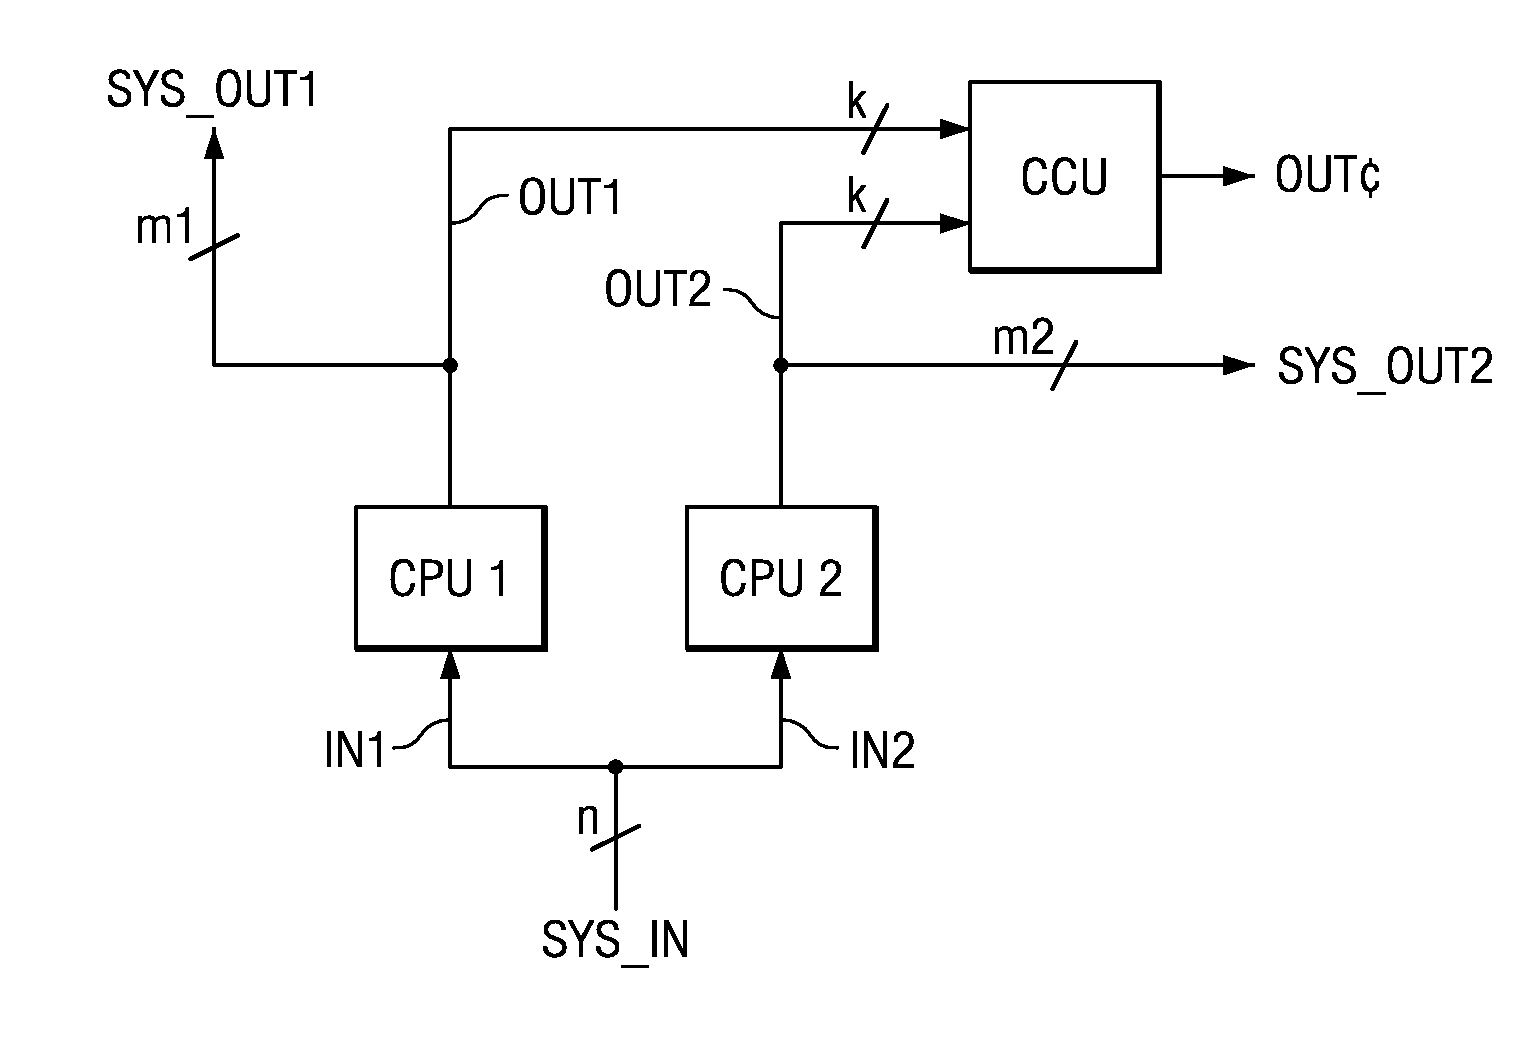
\includegraphics[width=0.9\linewidth]{images/patent_not_delayed.png}
      \caption{Block diagram of two processors in lockstep}
      \label{fig:patent_not_delayed}
    
\end{figure}

One approach in categorizing errors detectable by lockstep is soft and hard errors. Soft errors describe errors that happen by a temporary anomaly, e.g., electrostatic discharge (ESD), radioactive decay, cosmic radiation. These errors lead to unintended transient signals or conditions in CPU or in peripherals. Their lifetime is usually 2 milliseconds or less. This kind of error can affect an instruction execution or computation, but
the next time that the same operation will be performed the error will not be reproducible. On the other hand, hard errors are permanent and are caused by the
long term degradation of the silicon/logic over time. Hard errors may also occur
by corrupted memory cells or other circuit components due to ionizing radiation,
manufacturing inconsistencies, or exposure to a high current which may cause
metal migration. Generally, they are caused by a physical defect of the hardware and
they are not recoverable.

Lockstep architecture can detect the aforementioned soft and hard faults. If three processors are in lock-step, they are also fault-tolerant \citep{lockstep_analysis}. 

The processors in lock-step can get up to SIL3, but not SIL4 as the use of on-chip redundancy is limited by IEC 61508 standard to SIL3. Therefore, although it may seem, lockstep is certainly not a panacea in all safety systems, and a certain amount of work is needed to justify its usage. Nevertheless, for all safety integrity levels, but SIL4 lockstep is often used extensively (e.g. automotive applications) \citep{ipavic_lockstep}. 

\subsection{Delayed lockstep}
 
To battle the transient errors (soft errors) e.g. cosmic radiation that leads the CPU or peripherals into unintended states delayed lockstep was invented by Texas Instruments. One of the CPUs' input is delayed, while the other one's output is delayed ensuring that if a transient error happens it will not affect both CPUs on the same instructions \citep{patent_delayed_lockstep}. \autoref{fig:patent_delayed} visualizes the delayed lockstep.

\begin{figure}[H]

      \centering
      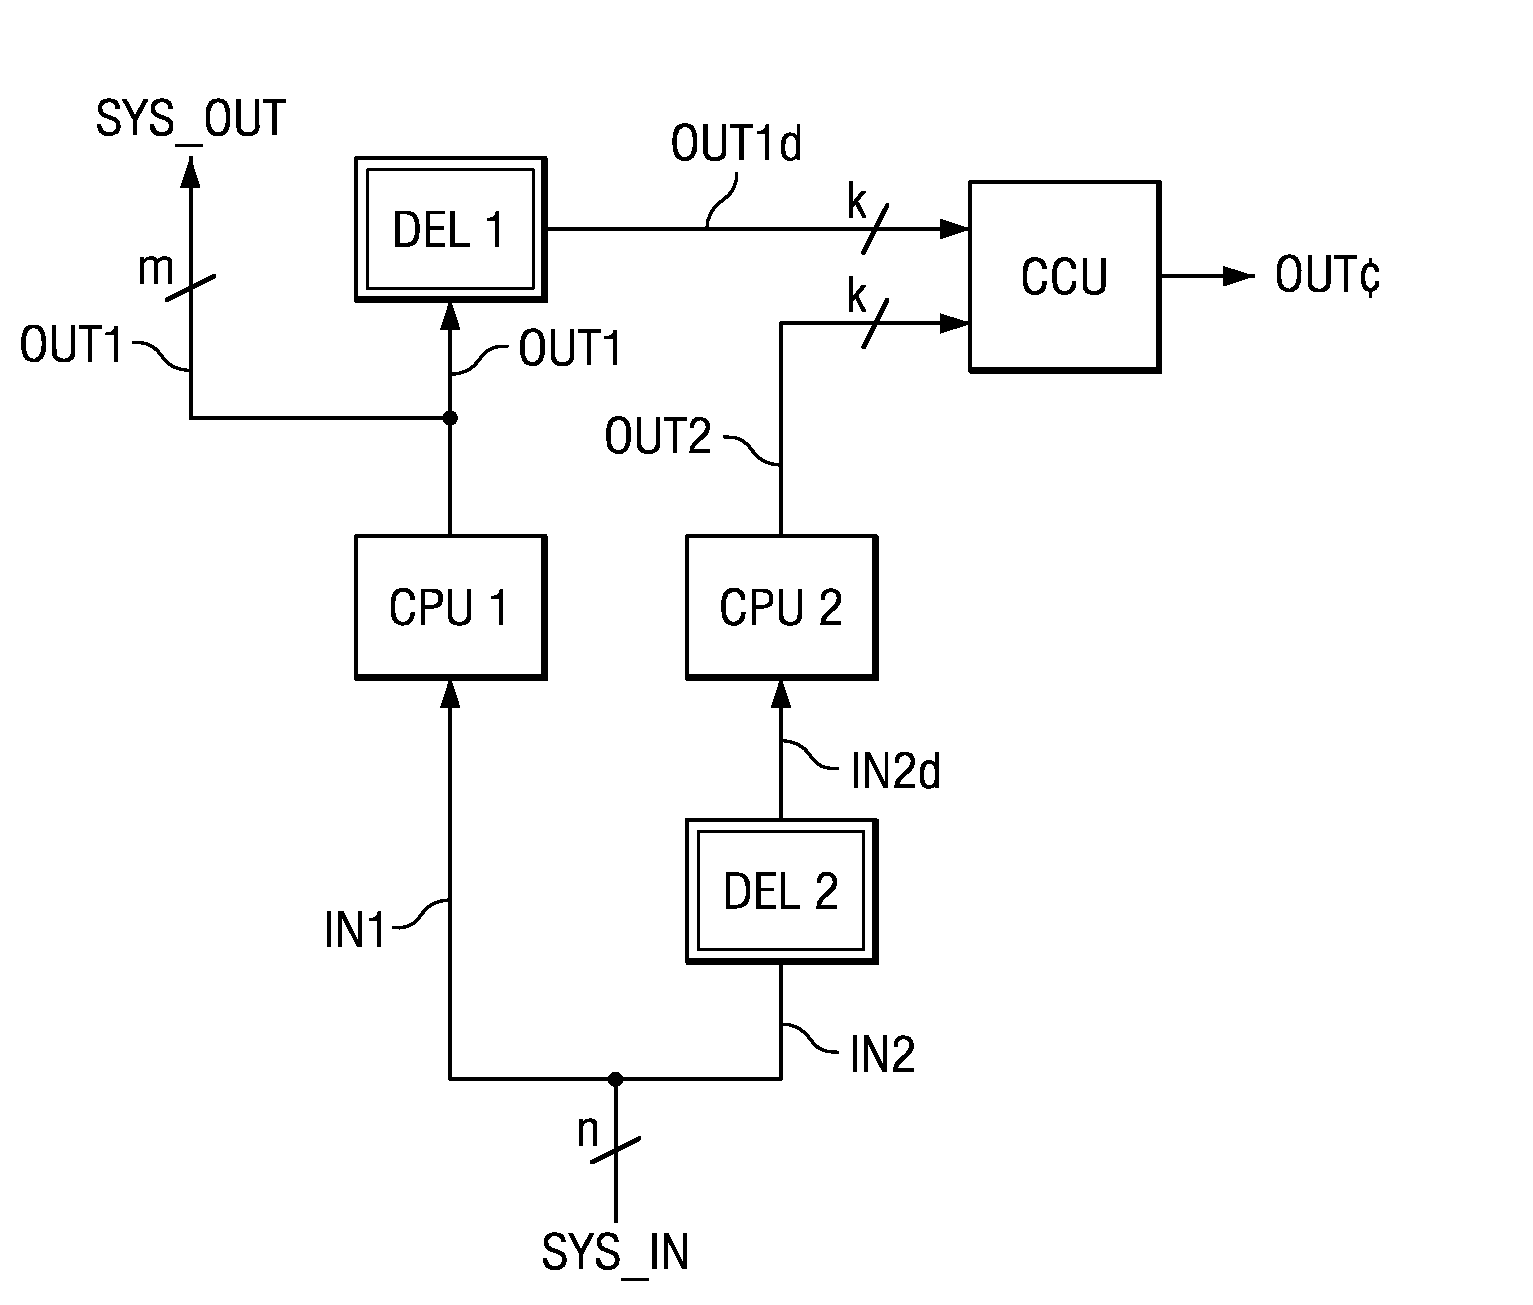
\includegraphics[width=0.8\linewidth]{images/patent_delayed.png}
      \caption{Block diagram of two processors in delayed lockstep}
      \label{fig:patent_delayed}
    
\end{figure}

\subsection{Positional diversity}

When designing lockstep architecture positional diversity shall also be considered. Two cores shall be rotated 90 degrees and flipped in relation to each other. At least 100 um space is left in between them. Physical diversity gives some assurance of a different failure mechanism if
there is a manufacturing flaw causing physical damage to the die. \autoref{fig:lockstep_cpu_position} visualizes an example of two cores on the silicon. ž

\begin{figure}[H]

      \centering
      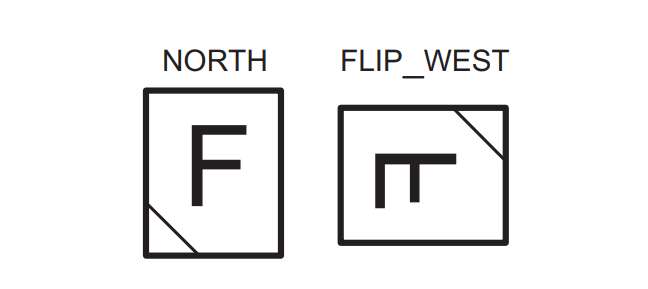
\includegraphics[width=0.8\linewidth]{images/lockstep_cpu_position.png}
      \caption{Typical orientation of the cores \citep{safety_maual_tms570ls31x}}
      \label{fig:lockstep_cpu_position}
    
\end{figure}

The common cause failures
that physical diversity is called to restrict might be due to manufacturing flaws
or even susceptibility to radiation due to the direction of some of the components
used in the core design. A simple example for a potential manufacturing flaw that
might be common to both cores without the physical diversity, suppose that there
is a geometry of a certain component that was prone to collecting moisture and it was processed in a way that this component was traveling parallel to some chemical spray in the process. This might lead to trapped materials at this component
in the silicon but if the components were rotated and flipped it would make the
likelihood of trapping contaminates less likely. In this way, making the two cores
physically diverse can keep both cores from having the same defective component \citep{lockstep_analysis}. 

\subsection{Debugging}

During a debug session, where the execution of the code is halted, several asynchronous halting events occur, with a possibility to lead to a loss of Lockstep (an indication of non-existing errors). For this reason, when halting debug events are
detected, the compare unit is automatically disabled. In order to set the Lockstep
mode on and the compare unit in the operational state, a CPU reset is required. \citep{TMS570LS31x21x_manual}

\subsection{Example use case}

A simplified example application is covered in this subsection to better explain the benefits of the lockstep. It should be noted that without a prior functional-hazard analysis this is not an optimal use case.

Besides the fact that the rate of aircraft engine failures has dramatically decreased,
to the point that flight crews most likely will not ever meet one in their
whole career, it still remains a possibility. Because of this infrequent occurrence
of an engine failure the crew is not always able to identify and to handle such a
malfunction. As a result, erroneous operations of the crew in such a case could
lead to devastating consequences for them and for the passengers.

The likely most complex and crucial component on an airplane is the engine. The main part of the safety relies on this component. In this example, we will focus on the fire detection scenario of the engine. 
In avionics, there is the principle of keeping the aircraft trajectory as
the highest priority duty [9]. Thus, in case of an engine malfunction, the system
should stabilize the aircraft trajectory first, before proceeding with further actions
to resolve the engine problem. This could probably cause larger damage to the
engine but it would help to ensure the safety of humans and the aircraft itself  \citep{lockstep_analysis}.

One of the functions of the engine's single-core MCU is to receive the raw values from temperature sensors, making sense of them and notifying the crew if the temperature is too high to prevent fire.  
After taking the appropriate actions to stabilize the aircraft trajectory (i.e activate a redundant engine) the system sets the defective engine to the idle state. In high
altitude the level of radiation that occurs from cosmic rays is significantly high.
Such radiation can cause a bit flip in the core of the
system that executes this temperature calculation. If the bit flip happens during the conversion of the raw values a spurious alarm could be raised. The erroneous calculation could end up in a non-realistic
over-limit temperature value, leading to an undesirable deactivation of the engine
and getting the flight crew into trouble. One can conclude, Single-core MCU can not detect an error in the context of executing the commands  \citep{lockstep_analysis}.

If in place of a single-core MCU, a lock-step MCU with two cores is placed such error would be detected and could temporarily set the system in a safe-state. The
two cores operating in Lockstep, most likely would not experience the same bit-flip
and they would produce divergent outputs. This discrepancy in the comparison of
the output signals would generate an error.


From the error detection, the implementation differs according to the system requirements. For instance, if the system could handle to “wait” the time that is required for a
soft-reset of the MCU, it could be determined if the error is temporal or permanent.
In case of a permanent error, the system could finally set the engine idle and enable
a redundant one. In case of a soft error, a reset of the system could be enough to
continue operating efficiently.


